\section{Neural network based caching policy} \label{caching_policy}

\subsection{Architecture} \label{architecture}

\begin{figure}[b!]
	\centering
	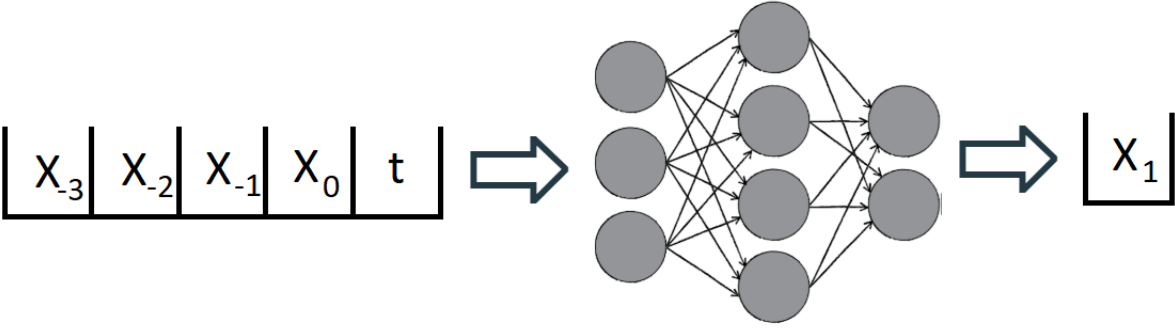
\includegraphics[width=\linewidth]{pics/cache1.png}
	\caption{Neural network architecture for caching policy.}
	\label{fig:cache1}
\end{figure}

Following the success in the application of a neural network for object popularity predictions, we are proposing a neural network based caching policy. On the Figure \ref{fig:cache1} you can see the proposed usage of the neural network by the policy.

\begin{itemize}
	\item $X_{-3}$ through $X_{-1}$ are popularities of the object in the previous 3 time frames;
	\item $X_0$ is the popularity of the object in the current time frame;
	\item $t$ is the fraction of the current time window that has already passed;
	\item $X_1$ is the popularity of the object in the future;
\end{itemize}

As you can see, the architecture of the neural network is slightly different from the one described in the previous section.  The difference is caused by the nature of the application of caching policies. The policy is working in the real-time thus we cannot operate in the framework of only previous and next time frames. $X_0$ represents the popularity in the current time frame. But at the beginning of the time frame, the quality of the value $X_0$ may be low since there will not be enough requests in the time window to estimate the popularity with reasonable accuracy. To help with this issue, we decided to add the parameter $t$. Using this parameter, the neural network will be able to learn to judge the quality of the parameter $X_0$ and make better predictions. Further, we will also experiment with different number of prediction windows and trying to add other metadata to improve the accuracy of predictions.

\begin{figure}[t!]
	\centering
	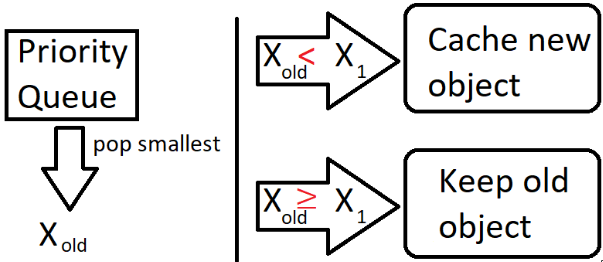
\includegraphics[width=0.75\linewidth]{pics/cache2.png}
	\caption{Usage of prediction by the policy.}
	\label{fig:cache2}
\end{figure}

After the prediction is made, the value $X_1$ is used to decide if the object should be put in the cache. The policy maintains a priority queue in which the key of each entry is the predicted popularity, and the values are IDs of the objects currently stored in the cache. When a new object is requested, and it has not been stored in the cache, the neural network predicts the popularity of the object in the future - $X_1$. Then, an object with the smallest predicted popularity is fetched from the priority queue, and its popularity is denoted as $X_{old}$. If the value $X_1$ is greater than $X_{old}$, then the old object is removed from the cache, and the new one is put in its place and into the priority queue. Otherwise, no change occurs. 

With this design, a problem may arise - if the prediction of popularity for some object has been calculated to be very high, it may never be removed from the cache since it will never be fetched for replacement. A solution to this problem is to update the priority for a few random objects stored in the cache with each cache hit.

\begin{figure}[t!]
	\centering
	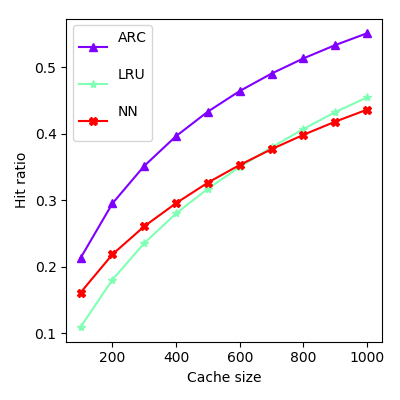
\includegraphics[width=0.5\linewidth]{pics/cache3.png}
	\caption{Poor performance of the first version.}
	\label{fig:cache3}
\end{figure}

Also, the value $X_1$ requires a better explanation. Trying to predict the popularity of the object in the next time frame, as in the previous offline case, did not show good performance when evaluating the hit rate, as seen on the Figure \ref{fig:cache3}. The identified problem was that the prediction was made too far in the future. The influence of the issue can be summarized in two cases:

\begin{enumerate}
	\item If the object is popular in the current time window but then gets unpopular in the next, it wouldn't be put into the cache, but since the current time window is not finished, and the object is still popular, a lot of cache misses will occur.
	\item The opposite problem - when the object is not popular but then gets popular. This object will take a place in the cache even though it is not popular yet.
\end{enumerate}

To resolve this issue, we changed the scope of the value $X_1$. The desirable performance has been achieved with when $X_1$ represents the popularity at the end of the current time frame and displayed on the Figure \ref{fig:cache4}. Probably it is still possible to improve the performance by fine tuning the parameters. 

\begin{figure}[h!]
	\centering
	\begin{subfigure}[b]{0.49\linewidth}
		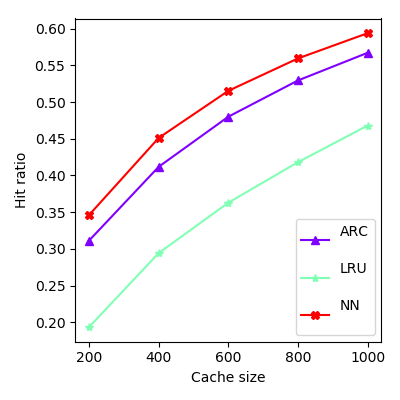
\includegraphics[width=\linewidth]{pics/cache4.png}
		\caption{5-day trace.}
	\end{subfigure}
	\begin{subfigure}[b]{0.49\linewidth}
		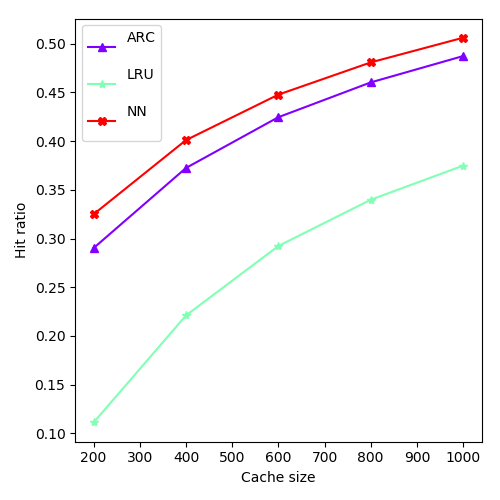
\includegraphics[width=\linewidth]{pics/cache4_2.png}
		\caption{30-day trace.}
	\end{subfigure}
	\caption{Improved performance of the policy.}
	\label{fig:cache4}
\end{figure}

\subsection{Online learning} \label{online_learning}

One of the most important parts of a caching policy is to be able to perform well in different environments with different traffic patterns. That is why it is important to make the policy adaptable. In our case, such adaptability is provided by the ability of the neural network to continuously evolve by training on the newly arrived data. After the end of each time frame, it is possible to generate a new training dataset and use it to train the neural network, possibly asynchronously. But by training only on the latest data, we may encounter the problem of catastrophic forgetting\cite{16, 17}. In short, the issue is that by training only on the latest data the neural network will forget the information about the old underlying relations between input and output even though they still may be relevant for predictions. 

To overcome this issue, we incorporate a technique of keeping the training datasets of previous time frames and training the neural network also on them. But since they represent less relevant data, the error, which is backpropagated during the training of the neural network, is scaled down with a parameter $\alpha^M \text{, where } 0 < \alpha < 1 \text{ and } M$ - is the distance from current time frame to previous time frames. In this way, the error on the latest data will stay unchanged since the value of $M$ is $0$. Moving further in the past $\alpha^M \rightarrow 0$ and the influence of the old data is reduced. When $\alpha^M$ reaches some small value, the old training data becomes too irrelevant and can be removed from the memory. Using this approach with the value of $\alpha = 0.5$ and forget threshold of $0.001$ it is required to store training datasets generated only for $10$ latest time frames while keeping the predictions made by the neural network accurate and relevant.

\subsection{Parameter selection} \label{parameter_selection}

Having achieved good performance on the real 5-day trace and overperforming state of the art policy ARC on all cache sizes, as seen in the Figure \ref{fig:cache4}, even without giving much consideration to the parameters of the proposed policy, it is time to explore the optimal ways to select the parameters.

\begin{figure}[t!]
	\centering
	
	\begin{subfigure}[b]{0.49\linewidth}
		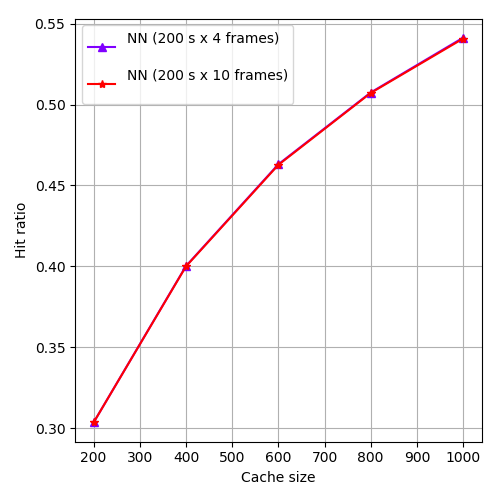
\includegraphics[width=\linewidth]{pics/cache5.png}
		\caption{5-day trace.}
	\end{subfigure}
	\begin{subfigure}[b]{0.49\linewidth}
		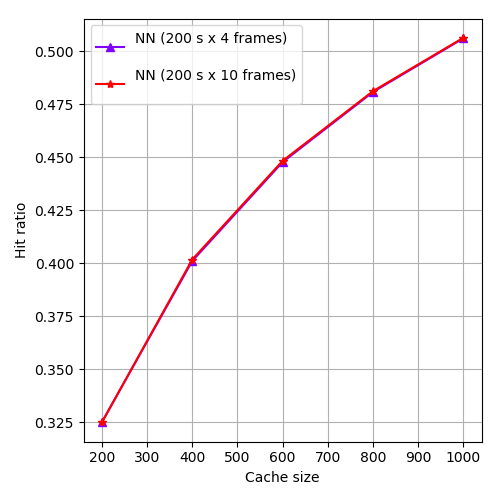
\includegraphics[width=\linewidth]{pics/cache5_2.png}
		\caption{30-day trace.}
	\end{subfigure}
	\caption{Comparison of performance with larger number of time frames.}
	\label{fig:cache5}
\end{figure}

The first step we decided to check is the required number of time windows. To establish this experiment, we have fixed the length of the time frame at the values of 200 seconds and tested two configurations - 4 time frames (3 previous + current) and 10 time frames (9 previous + current). The results of the experiment can be seen in the Figure \ref{fig:cache5}. As seen in the figure, the cache hit ratio values coincide for each tested cache size. From this, we can conclude that it is enough to use 4 time frames for popularity predictions and there is no point in increasing this number.


Following this, we have to determine the optimal way to select the length of the time frame. We have established an experiment trying to evaluate this value. Parameters of the experiment:

\begin{itemize}
	\item Time frame sizes: 3 s, 10 s, 50 s, 200 s, 1000 s.
	\item Cache sizes: 200, 400, 600, 800, 1000.
	\item Trace length: first 50 000 000 requests from both of real traces.
\end{itemize}

\begin{figure}[t!]
	\centering
	
	\begin{subfigure}[b]{0.49\linewidth}
		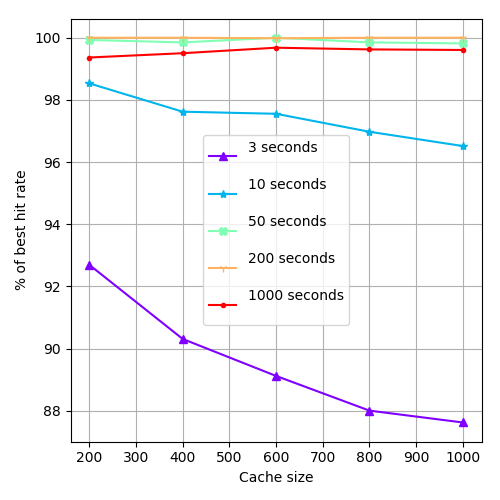
\includegraphics[width=\linewidth]{pics/cache6.png}
		\caption{5-day trace.}
	\end{subfigure}
	\begin{subfigure}[b]{0.49\linewidth}
		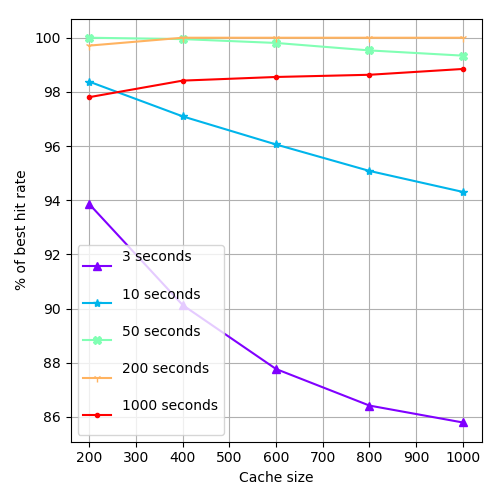
\includegraphics[width=\linewidth]{pics/cache6_2.png}
		\caption{30-day trace.}
	\end{subfigure}
	\caption{Comparison of performance with different size of time frame.}
	\label{fig:cache6}
\end{figure}

The experiment showed that the size of the window influences more on the performance than the number of windows. For both traces, the size of 200 s showed the best performance for all cache sizes with the exception of cache size 200 on the 30-day trace, as you can observe on the Figure \ref{fig:cache6}. The figure shows the ratio between the hit ratio of the best performing time frame size and all of the others. From this, we can propose a rule of thumb for selecting the size of the time frame for the policy. It is reasonable to assume that the lower the request rate the higher the size of the time frame should be, since with fixed length of the time frame and decreasing request rate the accuracy of the estimation of the popularity of the objects also decreases. Both traces have approximately 900 requests/s request rate and show the best performance at the size of the window of 200 s. Thus, the rule of thumb is to select the size of the window such that the next equation holds true: $$ frame\_size * request\_rate \approx  180000 $$.

Another point to notice can be observed of the Figure \ref{fig:cache6} (b). As the cache size increases, the 50 second time frame policy is on the downward trend while 1000 second time frame is on the upward trend.  From this, we can conclude that the available size of the cache also should be accounted for when selecting the time frame size.

We are not claiming that the proposed rule is the best way to select the size of the time frame since in all cases the performance of the 50 second frame size was very close to the best performing size of 200 seconds, even overperforming it in one case but following the provided rule of thumb should give close to optimal results.

\subsection{Perspective improvements} \label{perspective_improvements}

\begin{figure}[b!]
	\centering
	
	\begin{subfigure}[b]{0.49\linewidth}
		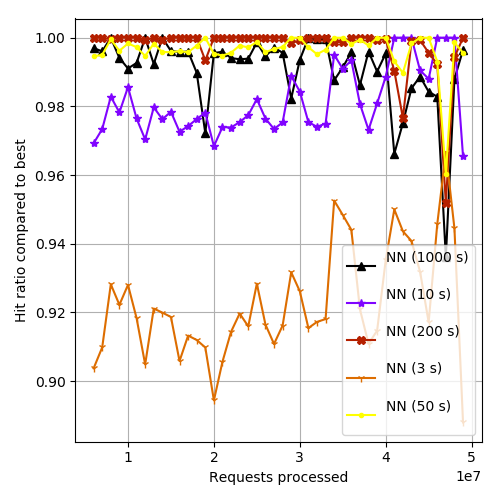
\includegraphics[width=\linewidth]{pics/cache7.png}
		\caption{5-day trace.}
	\end{subfigure}
	\begin{subfigure}[b]{0.49\linewidth}
		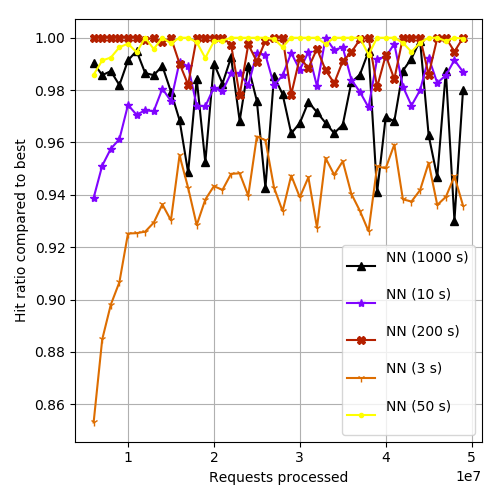
\includegraphics[width=\linewidth]{pics/cache7_2.png}
		\caption{30-day trace.}
	\end{subfigure}
	\caption{Comparison of immediate cache hit ratio for different time frame sizes.}
	\label{fig:cache7}
\end{figure}

Examining the cumulative hit rate revealed that the time frame size of 200 seconds performed the best. But studying closely the immediate hit rate, i. e. evaluating the hit rate after each million of requests rather than the total hit rate, revealed some interesting behavior. Figure \ref{fig:cache7} shows the ratio between the best-performing policy modification and other modifications evaluating immediate hit rate as described before for both of the real traces and cache size of 200. The figure reveals that the best-performing cumulatively time frame size does not perform the best at each point in time of the traces. At some segments of the traces, the 50 second size performs the best, what could be expected since this size was very close to the best-performing in all tests, but at some segments the size of 10 seconds performed the best. Examining the segments of the traces on which the size of 10 seconds performed the best revealed that the rate of requests was very high which allowed the 10 second modification to estimate the popularity of the objects with high accuracy while being the fastest to adapt to the changes since it naturally follows from the smaller size of the time frame. Such behavior suggests that possibly it is better to reject the concept of time-based time frames and switch to request count-based time frames, i. e. the time frame will not span a fixed amount of time but a fixed number of requests. Such an approach should remove the dependence on the request rate of the request trace and could allow simplifying the parameter selection for the policy. But in the report, we will not touch such a modification and leave it for the future research.

Our attempts to improve the quality of predictions made by the neural network by passing as input some metadata alongside with the popularity in previous time frames, in our case, it was the size of the object and artificially extracted time of the day, did not improve the performance of the policy. But the approach of adding metadata to the input of the neural network should not be discarded. It is possible that some other metadata could improve the quality of predictions and the performance of the caching policy as the consequence but search for such metadata is left for the future research.

\subsection{Comparison with other proposed solutions} \label{comparison}

We have shown before that our proposed caching policy overperformes well established and frequently used policy LRU and industry leader policy ARC by close to 12\% and 3\% in the cache hit ratio respectfully. But, as mentioned before, there are some proposed policies which also rely on machine learning algorithms for caching purposes. We have selected the approach proposed in \cite{23} to compare with the method proposed by us. As explained before, the policy proposed in \cite{23} applies deep long short-term memory network to determine the caching priority and decide which objects to store/remove in/from the cache. We have implemented the policy using the PyTorch library, which was also used to implement the neural network in our approach. DLSTM approach deals with a fixed number of items, so we filtered the 5-day trace to contain only $300 000$ most popular objects. After selecting the parameters of the policy as proposed by the author of \cite{23}, we evaluated the hit rate on our filtered trace. The produced hit rate values were less than 1\%. We reduced the number of unique items to 1000 and repeated the experiment, now with a better result shown in the Figure \ref{fig:dlstm}. The policy is showing some promise as can be seen by the upward trend in the cumulative cache hit ratio but the slow speed of adaptation at the first half of the trace caused a lower final cache hit ratio than achieved by ARC or our approach. Adding the disadvantage of a limited number of unique items to the slow adaptation speed of DLSTM policy we can claim that our approach is superior to the one proposed in \cite{23}.

\begin{figure}[t!]
	\centering
	
	\begin{subfigure}[b]{0.49\linewidth}
		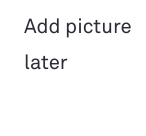
\includegraphics[width=\linewidth]{pics/todo.png}
		\caption{5-day trace.}
	\end{subfigure}
	\begin{subfigure}[b]{0.49\linewidth}
		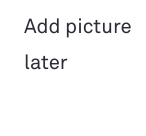
\includegraphics[width=\linewidth]{pics/todo.png}
		\caption{30-day trace.}
	\end{subfigure}
	\caption{DLSTM performance comparison.}
	\label{fig:dlstm}
\end{figure}